\section{Methodology}
\label{sec:method}

Fig.~\ref{fig:flow} summarises ToonSense. Text and image are encoded by frozen pretrained encoders, and a lightweight
head is trained on the cached embeddings for each task. Perturbations are injected \emph{before} the encoders, so the
same trained heads are evaluated on clean and perturbed versions of the same memes. Freezing the encoders keeps the
study affordable and ensures that a perturbation changes only the input, never the evaluated classifier.

\begin{figure*}[t]
  \centering
  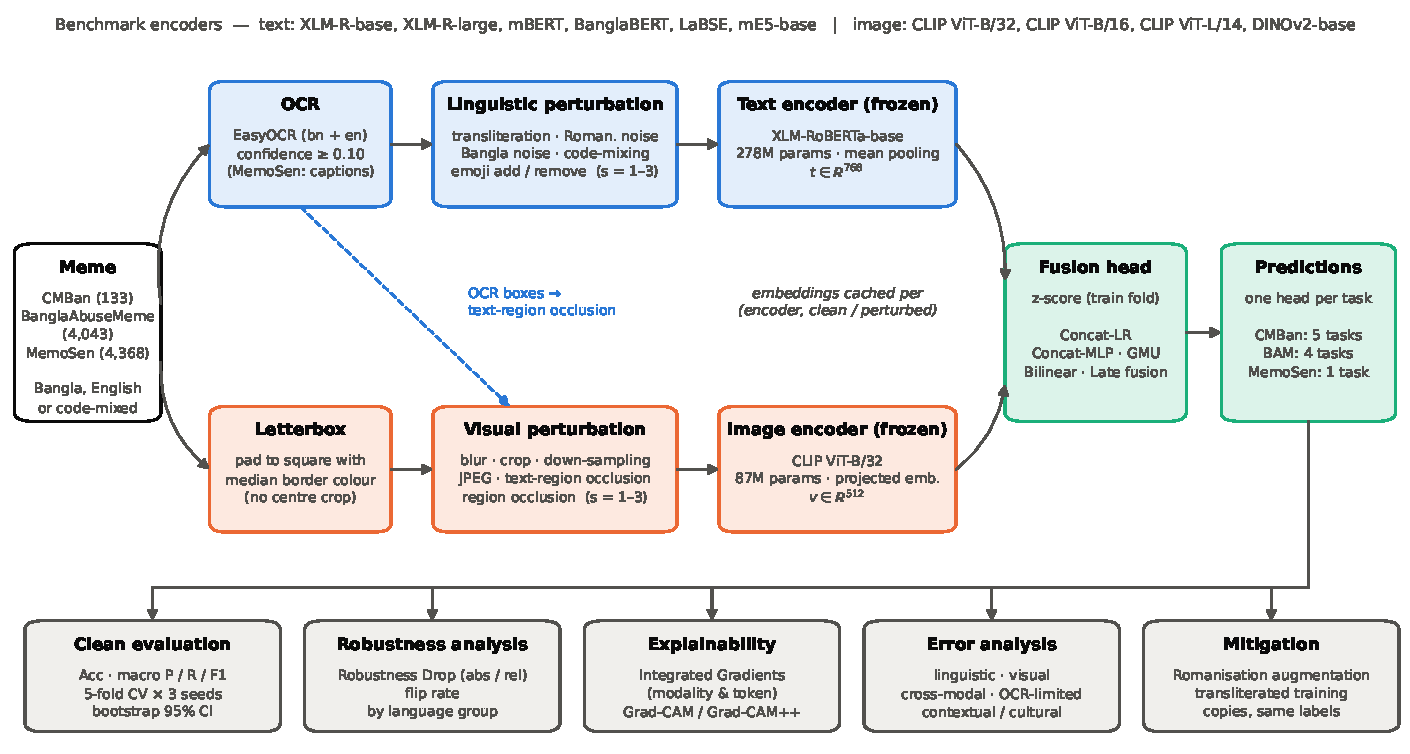
\includegraphics[width=\textwidth]{figures/methodology_flow.pdf}
  \caption{ToonSense pipeline. Meme text comes from OCR (MemoSen: human captions) and is encoded by XLM-R-base; the
  letterboxed image is encoded by CLIP ViT-B/32. Linguistic and visual perturbations ($s\in\{1,2,3\}$) are applied
  before the frozen encoders. Predictions feed the clean, robustness, explainability and error analyses, and a
  train-time augmentation tests a mitigation. Alternative encoders (top) are used in the benchmark.}
  \label{fig:flow}
\end{figure*}

\subsection{Datasets}
\label{sec:method:data}

Table~\ref{tab:datasets} lists the three datasets, which are processed \emph{separately}; only the protocol is
shared. CMBan~\cite{cmban2025} reports 2{,}641 memes, but labels are public for only 133 (85 Bangla, 45 code-mixed,
3 English). Because several fine classes are tiny, we use coarse labels that collapse intensity levels (e.g.\ funny
vs.\ not funny). To test whether findings hold at scale, we repeat the full protocol on
BanglaAbuseMeme~\cite{das2023banglaabusememe} (BAM), whose text is rendered in the image, and
MemoSen~\cite{hossain2022memosen}, which ships human-written captions and so removes OCR noise. Memes are grouped by
script as Bangla ($\geq$85\% Bangla letters), Latin-script ($\leq$15\%) or code-mixed.

\begin{table}[t]
\centering
\small
\caption{Datasets. Classes in parentheses (CMBan: fine/coarse).}
\label{tab:datasets}
\begin{adjustbox}{max width=\columnwidth}
\begin{tabular}{lrll}
\toprule
Dataset & $N$ & Tasks (classes) & Text \\
\midrule
CMBan & 133 & humour, sarcasm, offensive (3/2), & OCR \\
 & & motivational (2), sentiment (5/3) & \\
BAM & 4{,}043 & sentiment (3), sarcasm, abuse, vulgarity (2) & OCR \\
MemoSen & 4{,}368 & sentiment (3) & human \\
\bottomrule
\end{tabular}
\end{adjustbox}
\end{table}

\subsection{Encoders and Heads}
\label{sec:method:enc}

\textbf{Pre-processing.} Text is extracted with EasyOCR~\cite{easyocr} (Bangla+English); fragments with confidence
below 0.10 are dropped and the rest ordered in reading order. Mean OCR confidence is 0.58 (CMBan) and 0.54 (BAM).
Images are letterboxed to a square before encoding, so tall multi-panel comics are not cropped.

\textbf{Encoders.} The primary pair is XLM-RoBERTa-base~\cite{conneau2020xlmr} (mean-pooled, 768-d) and CLIP
ViT-B/32~\cite{radford2021clip} (512-d projection). For the benchmark we add XLM-R-large, mBERT~\cite{devlin2019bert},
BanglaBERT~\cite{bhattacharjee2022banglabert}, LaBSE~\cite{feng2022labse} and mE5-base~\cite{wang2024me5} as text
encoders, and CLIP ViT-B/16, ViT-L/14 and DINOv2-base~\cite{oquab2024dinov2} as image encoders. We chose the primary
pair for its coverage of Bangla, English and Romanised tokens in one vocabulary, its language-supervised image
features and its cost: CLIP-B/32 is the smallest image encoder, which matters because the robustness protocol
re-encodes 36 perturbed copies of every dataset.

\textbf{Heads.} Embeddings are standardised per training fold. Unimodal heads are an $\ell_2$-regularised logistic
regression (LR) and a two-layer MLP ($H=256$, GELU, dropout 0.3). Fusion heads are \emph{Concat-LR/MLP} on
$[\mathbf{t};\mathbf{v}]$; a \emph{GMU}~\cite{arevalo2017gmu},
$\mathbf{h}=\mathbf{z}\odot\tanh(W_t\mathbf{t})+(1-\mathbf{z})\odot\tanh(W_v\mathbf{v})$ with
$\mathbf{z}=\sigma(W_z[\mathbf{t};\mathbf{v}])$; a \emph{bilinear} head on
$[\mathbf{a};\mathbf{b};\mathbf{a}\odot\mathbf{b};|\mathbf{a}-\mathbf{b}|]$ of projected embeddings; and \emph{late
fusion}, averaging text- and image-MLP probabilities. Baselines are the majority class and a character 2--5-gram
TF-IDF + LR. Neural heads use AdamW ($10^{-3}$), class-weighted cross-entropy and early stopping (patience 30) on an
inner validation split, on which the LR regularisation $C\in\{0.01,0.1,1\}$ is also selected.

\subsection{Perturbations}
\label{sec:method:pert}

Table~\ref{tab:perturbations} lists six linguistic and six visual families. \emph{Transliteration} uses a rule-based
Bangla-to-Banglish converter written for this study that follows colloquial conventions (schwa deletion,
\textit{ya-}/\textit{ba-phala}); \emph{Romanised spelling noise} romanises fully and then applies common Banglish
variants (\textit{sh}$\leftrightarrow$\textit{s}, \textit{bh}$\to$\textit{v}, vowel dropping); \emph{Bangla spelling
noise} swaps confusable native characters; \emph{code-mixing} switches words with a $\sim$200-word bilingual lexicon.
\emph{Text occlusion} fills OCR boxes with their median colour, and \emph{region occlusion} greys out non-text grid
cells. Perturbations are deterministic per meme, family and severity. A linguistic perturbation changes only the text
input and a visual one only the image input, so each effect is attributable to one modality.

\begin{table}[t]
\centering
\small
\caption{Perturbation families; parameter at severity $s=1/2/3$.}
\label{tab:perturbations}
\begin{adjustbox}{max width=\columnwidth}
\begin{tabular}{lll}
\toprule
 & Family & $s=1/2/3$ \\
\midrule
\multirow{6}{*}{\rotatebox{90}{Linguistic}}
 & Transliteration  & 33/66/100\% of Bangla words \\
 & Roman.\ spelling noise & 15/30/50\% of words (after romanising) \\
 & Bangla spelling noise  & 10/20/35\% of Bangla words \\
 & Code-mixing      & switch prob.\ 0.33/0.66/1.0 \\
 & Emoji insertion  & 1/3/6 emojis \\
 & Emoji removal    & emojis / +emoticons / +symbols \\
\midrule
\multirow{6}{*}{\rotatebox{90}{Visual}}
 & Gaussian blur    & $\sigma$=1/2/4 (224-px scale) \\
 & Random crop      & 85/70/55\% of area kept \\
 & Down-sampling    & 160/96/48 px, then up-sampled \\
 & JPEG             & quality 30/15/5 \\
 & Text occlusion   & 33/66/100\% of OCR boxes \\
 & Region occlusion & 10/25/40\% of non-text area \\
\bottomrule
\end{tabular}
\end{adjustbox}
\end{table}

\subsection{Evaluation}
\label{sec:method:eval}

We use stratified 5-fold cross-validation repeated with three seeds; 15\% of each training fold is held out for
early stopping and model selection. Metrics are computed on out-of-fold predictions. Macro-F1 is the primary metric
because of class imbalance; we also report accuracy, 95\% bootstrap intervals, and paired bootstrap tests with Holm
correction across the tasks of a dataset~\cite{holm1979}. Each fold's model, trained on clean data, is applied to the
clean and the 36 perturbed versions (12 families $\times$ 3 severities) of its test fold. The relative
\emph{Robustness Drop} and the \emph{flip rate} are
\begin{align}
\mathrm{RD}&=100\cdot\frac{\mathrm{F1}(f;\mathcal{D})-\mathrm{F1}(f;\pi_s(\mathcal{D}))}{\mathrm{F1}(f;\mathcal{D})},\\
\mathrm{FR}&=\frac{1}{N}\sum_{i=1}^{N}\mathbf{1}\big[f(x_i)\neq f(\pi_s(x_i))\big].
\end{align}

\textbf{Mitigation.} To counter Romanisation without new labels, each non-validation training meme $i$ receives a copy
whose text is perturbed while image and label are kept,
$\mathcal{T}_{\text{aug}}=\mathcal{T}\cup\{(\pi_s(t_i),\mathbf{v}_i,y_i): i\in\mathcal{T}\setminus\mathcal{V},
\pi_s\in\Pi\}$. We compare no augmentation, \emph{+translit.} ($\Pi$ = transliteration, $s=2$; Romanised spelling
noise stays unseen) and \emph{+translit.\,+\,noise} (both families).

\textbf{Explainability.} Integrated Gradients~\cite{sundararajan2017ig} on the fusion input
$[\mathbf{t};\mathbf{v}]$ (training-mean baseline, 32 steps) gives the \emph{text share}
$\|\mathrm{IG}_\mathbf{t}\|_1/(\|\mathrm{IG}_\mathbf{t}\|_1+\|\mathrm{IG}_\mathbf{v}\|_1)$ of each decision.
Grad-CAM~\cite{selvaraju2017gradcam} on the CLIP patch tokens gives the \emph{text-attention ratio} (CAM mass inside
OCR boxes divided by their area share) and \emph{CAM stability} (correlation of clean and perturbed maps).

\textbf{Error taxonomy.} Comparing the best learned fusion head with the text- and image-MLP, a clean error is
\emph{linguistic} (only the text model wrong), \emph{visual} (only the image model wrong), \emph{cross-modal} (both
unimodal models right, fusion wrong), \emph{OCR-limited} (all wrong, OCR empty or confidence $<0.5$) or
\emph{contextual/cultural} (all wrong despite usable text). Late fusion is excluded because it cannot be wrong when both
unimodal models agree on the correct binary label.

\textbf{Implementation.} The pipeline uses PyTorch, Transformers, scikit-learn and EasyOCR. CMBan runs on a laptop
CPU; BAM and MemoSen took 4--6\,h each on a Kaggle Tesla T4. Code and perturbation generators are released.
